\documentclass[a4paper]{article}
\usepackage[utf8]{inputenc}
\usepackage[russian,english]{babel}
\usepackage[T2A]{fontenc}
\usepackage[left=10mm, top=20mm, right=18mm, bottom=15mm, footskip=10mm]{geometry}
\usepackage{indentfirst}
\usepackage{amsmath,amssymb}
\usepackage{mathastext} 
\usepackage[italicdiff]{physics}
\usepackage{graphicx}
%\usepackage{caption}
\usepackage{float}
\usepackage{caption}
\renewcommand{\thefootnote}{\fnsymbol{footnote}}
\usepackage{tablefootnote}
\usepackage{footmisc}
\usepackage{textcomp}
\usepackage{multicol}
\usepackage{multirow}
\usepackage[parfill]{parskip}
\usepackage{makecell}
\usepackage{array}  
\usepackage{siunitx}
\usepackage{booktabs}
\sisetup{
    exponent-product = \cdot,
    per-mode = symbol,
    separate-uncertainty = true,
    uncertainty-separator = \,
}
\renewcommand\cellalign{cc} 
\renewcommand\cellgape{\Gape[2pt]} 
\usepackage[utf8]{inputenc}\newcommand{\approxtext}[1]{\ensuremath{\stackrel{\text{#1}}{\approx}}}
\usepackage[colorlinks=true, urlcolor=blue, linkcolor=blue, citecolor=blue]{hyperref}
\graphicspath{{images/}}
\DeclareGraphicsExtensions{.pdf,.png,.jpg}
\usepackage{wrapfig}
\captionsetup{labelformat=empty}
\usepackage{caption}
\captionsetup[figure]{name=Рисунок}
\captionsetup[table]{name=Таблица}
%\usepackage{newtxtext,newtxmath} 
\title{\textbf{Отчет о выполнении лабораторной работы 4.5.3} \\[0.5em] \large\itshape Сканирующий интерферометр}
\date{}
\author{Котляров Михаил, Б01-402}

\begin{document}

\maketitle
	
\section{Введение}

\subsubsection*{Цель работы:} знакомство с устройством и работой газового лазера непрерывного действия, со спектральными характеристиками лазерного излучения, а также с устройством и принципом действия сканирующего интерферометра Фабри—Перо.


\subsubsection*{Оборудование и инструментальные погрешности}

\textbf{Гелий-неоновый лазер "Плазма" ГН-15-1}: длина волны любой модели $\lambda = 632,8$ нм\\
\textbf{сканирующий интерферометр Фабри—Перо}: $L = 65$ см,\\
\textbf{поляроид},\\
\textbf{пластинка $\lambda$/4},\\
\textbf{линза},\\
\textbf{электронный осциллограф},\\
\textbf{фотодиод}


\section{Экспериментальная установка}
\begin{figure}[h]
    \centering
    
\includegraphics[width=0.8\textwidth]{Pictures/setup.png}
    \caption{Рис. 1. Схема экспериментальной установки}
    \label{fig:setup}
\end{figure}
Схема экспериментальной установки изображена на рис. \ref{fig:setup}.
Излучение He–Ne-лазера проходит через поляризационную развязку Р и линзу Л и поступает на вход сканирующего интерферометра (СИ). Поляризационная развязка предотвращает попадание в лазер излучения, отразившегося от элементов 
 оптического тракта. Это излучение может существенно повлиять на работу лазера и даже привести к срыву генерации. Развязка состоит из поляроида и пластинки $\lambda$/4, главные направления которой установлены под углом 45$^\text{o}$ по отношению к разрешённому направлению поляроида. После развязки П свет приобретает циркулярную поляризацию (например, по правому кругу). При отражении от передней поверхности линзы, от зеркала сканирующего интерферометра и т.п. свет распространяется в обратном направлении в виде левополяризованной волны. Такая волна, пройдя через пластинку $\lambda$/4, вновь приобретает линейную поляризацию. Однако направление колебаний в этой волне оказывается перпендикулярным направлению разрешённых колебаний поляроида, поэтому до лазера отражённая волна не доходит. 

Линза Л служит для уменьшения расходимости пучка, поступающего на вход сканирующего интерферометра. Линза снабжена поперечными и продольными салазками для юстировки прибора на максимум сигнала. Излучение, прошедшее сквозь сканирующий интерферометр, поступает на фотодиод ФД. Напряжение с фотодиода через усилитель подаётся на вертикальный вход электронного осциллографа ЭО.

Лазер питается от блока питания БП-1, фотодиод и усилитель~---
от БП-2. Напряжение на пьезоэлемент сканирующего интерферометра
подаётся с блока питания БП-2 и регулируется ручкой 1.


\section{Ход работы и обработка результатов}

\subsection{Измерение ширины пиков и межмодового расстояния}
Перед началом измерений проведём юстировку оптической схемы согласно описанию установки. Добьёмся устойчивой осциллограммы, соответствующей одному–двум доплеровским контурам. Для определения ширины отдельной моды на полувысоте и расстояния между соседними модами используем линейку с миллиметровыми делениями. Измерения выполним несколько раз; результаты занесём в таблицы.

\begin{table}[h]
\centering

\begin{tabular}{|c|}
\hline
Ширина пика, мм \\
\hline
3 \\
\hline
3 \\
\hline
4 \\
\hline
\end{tabular}
\caption{Таблица 1. Измерение ширины пика на полувысоте}
\end{table}

\begin{table}[h]
\centering

\begin{tabular}{|c|}
\hline
Расстояние между модами, мм \\
\hline
22 \\
\hline
24 \\
\hline
23 \\
\hline
\end{tabular}
\caption{Таблица 2. Измерение межмодового расстояния}
\end{table}

\begin{figure}[h]
    \centering
    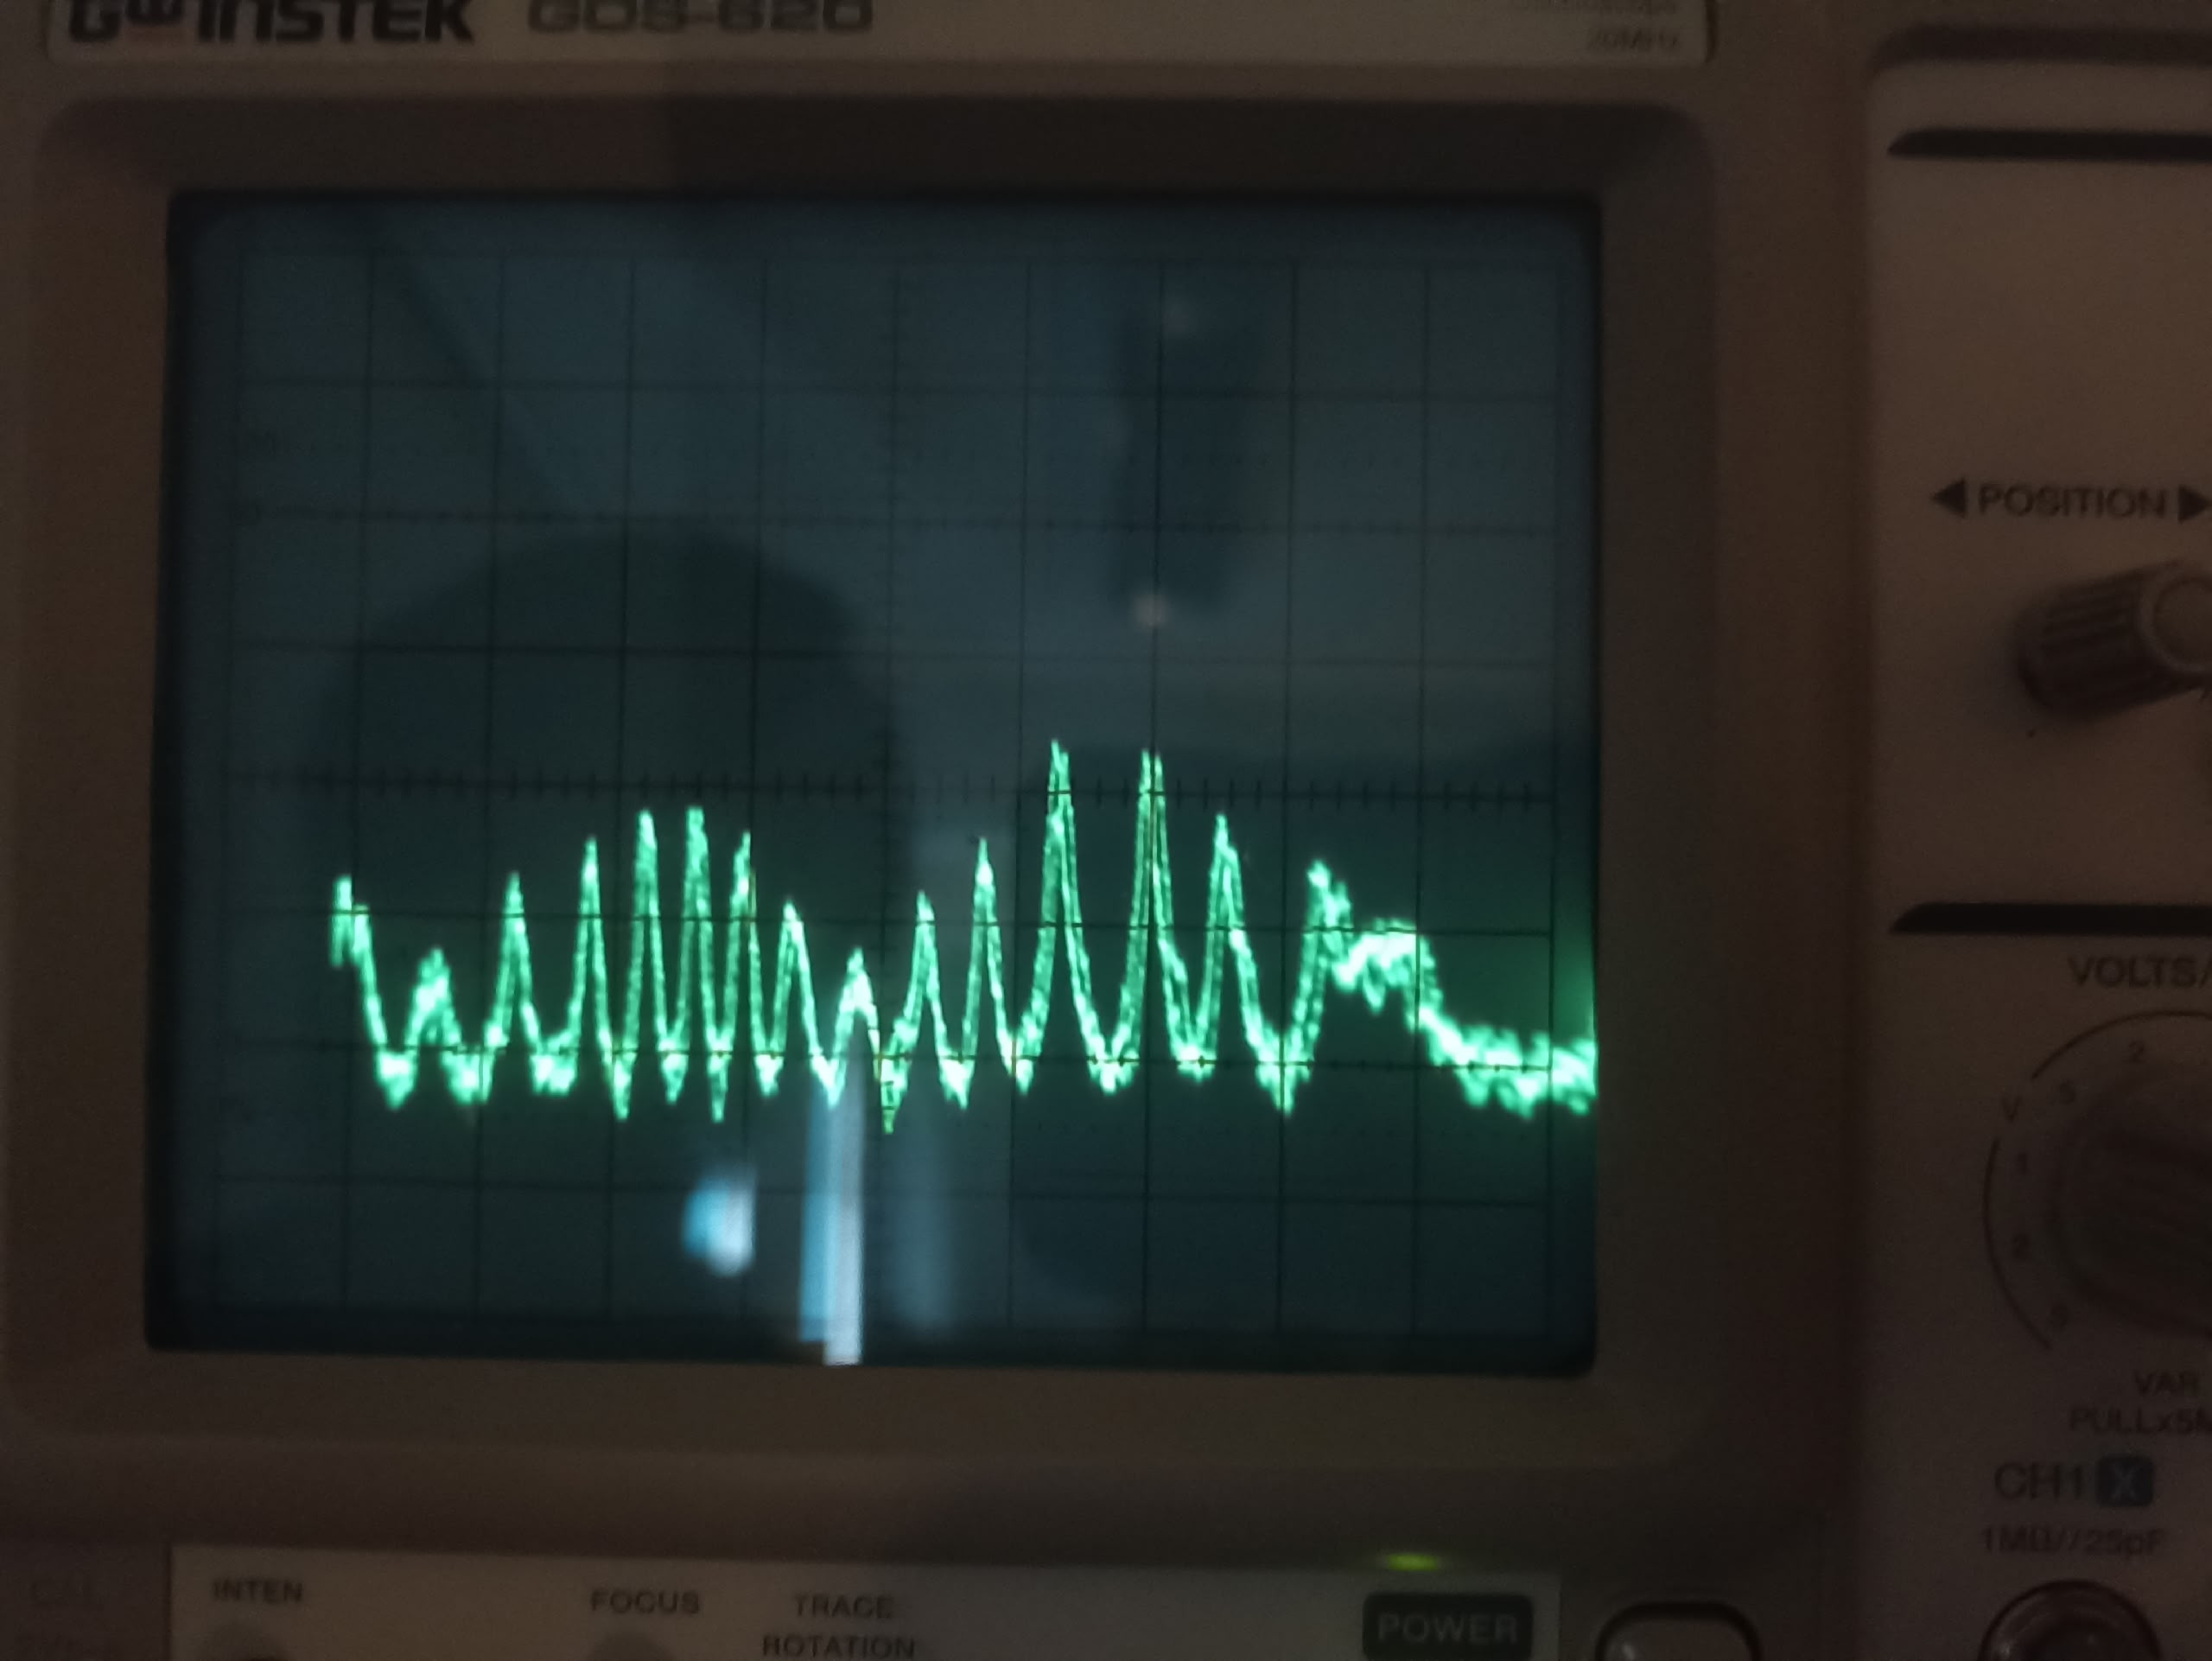
\includegraphics[width=0.8\textwidth]{Pictures/scope.jpg}
    \caption{Рис. 2. Спектр лазера}
    \label{fig:setup}
\end{figure}

Вычислим средние значения и случайные погрешности. Для ширины пика:
\[
\overline{h} = \frac{3+3+4}{3} = 3{,}333\ \text{мм},\qquad
\sigma_{h,\text{случ}} = \sqrt{\frac{\sum (h_i-\overline{h})^2}{n(n-1)}} = 0{,}333\ \text{мм}.
\]
Для межмодового расстояния:
\[
\overline{X} = \frac{22+24+23}{3} = 23{,}000\ \text{мм},\qquad
\sigma_{X,\text{случ}} = 0{,}577\ \text{мм}.
\]

Систематическая погрешность линейки составляет $\Delta_{\text{сист}} = 1$ мм. Полную погрешность найдём как корень квадратный из суммы квадратов случайной и систематической погрешностей:
\[
\Delta h = \sqrt{0{,}333^2 + 1^2} = 1{,}054\ \text{мм},\qquad
\Delta X = \sqrt{0{,}577^2 + 1^2} = 1{,}155\ \text{мм}.
\]

\subsection{Расчёт межмодового расстояния}
Исходные данные для расчётов сведём в таблицу.

\begin{table}[h]
\centering
\caption{Параметры установки}
\begin{tabular}{|c|c|c|c|c|c|c|}
\hline
$L$, см & $c$, см/с & $\lambda$, нм & $m_{\text{Ne}}$, а.е.м. & $1$ а.е.м., г & $k_{\text{Б}}$, эрг/К & $l$, см \\
\hline
$65 \pm 1$ & $3{,}000\cdot10^{10}$ & 632,8 & 20,2 & $1{,}66\cdot10^{-24}$ & $1{,}3806\cdot10^{-16}$ & 9 \\
\hline
\end{tabular}
\end{table}

Межмодовое расстояние резонатора лазера определим по формуле:
\[
\Delta\nu_{\text{мод}} = \frac{c}{2L},
\]
где $L = 0{,}65$ м, $c = 3\cdot10^8$ м/с. Получили:
\[
\Delta\nu_{\text{мод}} = (2{,}308 \pm 0{,}036)\cdot10^8\ \text{Гц}.
\]

\subsection{Определение ширины спектра генерации}
На осциллограмме зафиксировано $m = 7$ межмодовых интервалов на протяжении доплеровского контура. Полная ширина спектра в частотах:
\[
\Delta\nu_{\text{Ne}} = m \cdot \Delta\nu_{\text{мод}} = (1{,}615 \pm 0{,}025)\cdot10^9\ \text{Гц}.
\]
Пересчитаем в шкалу длин волн:
\[
\Delta\lambda_{\text{Ne}} = \frac{\lambda^2}{c}\,\Delta\nu_{\text{Ne}} = (2{,}156 \pm 0{,}033)\cdot10^{-3}\ \text{нм}.
\]

\subsection{Оценка скорости атомов и газокинетической температуры}
Используя упрощённые формулы лабораторной работы:
\[
\frac{\Delta\lambda_{\text{Ne}}}{\lambda} \approx \frac{v_x}{c},\qquad \frac{m_{\text{Ne}} v_x^2}{2} \approx \frac{kT}{2},
\]
найдём проекцию скорости $v_x$ и температуру $T$:
\[
v_x = c\cdot\frac{\Delta\lambda_{\text{Ne}}}{\lambda} = (1{,}022 \pm 0{,}016)\cdot10^5\ \text{см/с} = (1{,}022 \pm 0{,}016)\cdot10^3\ \text{м/с},
\]
\[
T = \frac{m_{\text{Ne}} v_x^2}{k_{\text{Б}}} = 2538 \pm 78\ \text{К}.
\]

Для учёта точного выражения доплеровской полуширины (гауссов контур) воспользуемся формулой:
\[
\frac{\Delta\lambda_D}{\lambda} = \frac{1}{c}\sqrt{\frac{8kT\ln 2}{m_{\text{Ne}}}}.
\]
Выразим $T$:
\[
T = \frac{m_{\text{Ne}} c^2}{8k\ln2}\left(\frac{\Delta\lambda_{\text{Ne}}}{\lambda}\right)^2 = 458 \pm 14\ \text{К}.
\]
Результат $458\ \text{К}$ соответствует типичным значениям газокинетической температуры в разряде He-Ne лазера.

\subsection{Дисперсионная область сканирующего интерферометра}
База интерферометра $l = 9$ см. Дисперсионная область:
\[
\Delta\lambda_{\text{СИ}} = \frac{\lambda^2}{2l} = 2{,}225\cdot10^{-3}\ \text{нм}.
\]

\subsection{Определение разрешающей способности интерферометра}
Ширину отдельной моды на полувысоте $\delta\lambda$ найдём путём калибровки осциллограммы по известному межмодовому расстоянию:
\[
\delta\lambda = \Delta\lambda_{\text{мод}} \cdot \frac{\overline{h}}{\overline{X}} = \frac{\lambda^2}{2L}\cdot\frac{\overline{h}}{\overline{X}}.
\]
Подставляя $\overline{h}=3{,}333$ мм, $\overline{X}=23{,}000$ мм:
\[
\delta\lambda = (4{,}46 \pm 1{,}43)\cdot10^{-5}\ \text{нм}.
\]

Разрешающая способность интерферометра:
\[
R = \frac{\lambda}{\delta\lambda} = (1{,}418 \pm 0{,}454)\cdot10^7.
\]

\subsection{Оценка коэффициента отражения зеркал}
Из формулы разрешающей способности интерферометра Фабри–Перо:
\[
R = \frac{2\pi l}{\lambda(1-r)},
\]
выразим $r$:
\[
r = 1 - \frac{2\pi l}{\lambda R} = 0{,}937 \pm 0{,}020.
\]
Полученное значение $r\approx0{,}94$ характерно для зеркал, используемых в сканирующих интерферометрах.

\section{Результаты и обсуждение}

В ходе эксперимента получены следующие количественные характеристики спектрального состава излучения He-Ne лазера и параметров сканирующего интерферометра Фабри–Перо.

\subsection{Межмодовое расстояние и ширина контура усиления}
Межмодовое расстояние составило $\Delta\nu_{\text{мод}} = (2,308 \pm 0,036)\cdot10^8$ Гц. Относительная погрешность $\approx 1,5\%$ обусловлена в основном погрешностью измерения $L$ и нестабильностью развёртки осциллографа.

Ширина спектра генерации (доплеровский контур) составила $\Delta\lambda_{\text{Ne}} = (2,156 \pm 0,033)\cdot10^{-3}$ нм, что соответствует $\Delta\nu_{\text{Ne}} = (1,615 \pm 0,025)$ ГГц. При $L = 0,65$ м межмодовое расстояние $\Delta\nu_{\text{мод}} \approx 231$ МГц, поэтому на ширине контура укладывается $7$ межмодовых интервалов (или $8$ мод). Это типично для He-Ne лазера с длиной резонатора около $0,6$–$0,7$ м и подтверждает, что ширина контура усиления ($\approx 1,5$ ГГц) значительно превышает $\Delta\nu_{\text{мод}}$, что и приводит к многомодовому режиму генерации.

\subsection{Температура разряда}
По упрощённой формуле работы получена завышенная температура $2538 \pm 78$ К, что является следствием отсутствия в ней множителя $\sqrt{2\ln 2}$ для полуширины гауссова контура. Корректная формула для доплеровской полуширины:
\[
\frac{\Delta\lambda_D}{\lambda} = \frac{1}{c}\sqrt{\frac{8kT\ln2}{m}},
\]
использование которой даёт $T = 458 \pm 14$ К. Это значение хорошо согласуется с типичными газокинетическими температурами в положительном столбе тлеющего разряда He-Ne лазера (обычно $400$–$600$ К). Относительная погрешность $\approx 3\%$ обусловлена погрешностью измерения $\Delta\lambda_{\text{Ne}}$.

\subsection{Дисперсионная область интерферометра}
Рассчитанная дисперсионная область $\Delta\lambda_{\text{СИ}} = 2,225\cdot10^{-3}$ нм. Она немного превышает измеренную ширину контура $\Delta\lambda_{\text{Ne}} = 2,156\cdot10^{-3}$ нм, что гарантирует наблюдение всего доплеровского контура в одном порядке интерференции без перекрытия порядков. Выбранная база интерферометра $l = 9$ см является оптимальной для данной задачи.

\subsection{Разрешение и коэффициент отражения}
Разрешение интерферометра (ширина аппаратной функции) составило $\delta\lambda = (4,46 \pm 1,43)\cdot10^{-5}$ нм, что соответствует разрешающей способности $R = (1,418 \pm 0,454)\cdot10^7$. Высокое значение $R$ позволяет уверенно различать соседние продольные моды лазера, расстояние между которыми $\Delta\lambda_{\text{мод}} = 3,34\cdot10^{-4}$ нм. Отношение $\Delta\lambda_{\text{мод}} / \delta\lambda \approx 7,5$, что значительно превышает критерий Рэлея и обеспечивает надёжное разрешение.

Коэффициент отражения зеркал интерферометра $r = 0,937 \pm 0,020$ близок к паспортным данным (обычно $r \approx 0,95$–$0,98$ для таких приборов). Небольшое занижение может быть связано с погрешностью измерения ширины пика $\delta\lambda$, а также с возможным загрязнением зеркал или остаточными потерями на пропускание и рассеяние.

\subsection{Анализ погрешностей}
Основной вклад в погрешность измерения $\delta\lambda$ (а следовательно, $R$ и $r$) вносит систематическая погрешность линейки ($\pm1$ мм) при определении ширины пика и межмодового расстояния на экране осциллографа. Случайная составляющая мала (коэффициент вариации около $10\%$ для ширины пика и $2,5\%$ для межмодового расстояния). Относительная погрешность $\delta\lambda$ достигла $32\%$, что вполне допустимо для учебной лабораторной работы, поскольку порядок величины определён верно, а основные физические выводы остаются справедливыми.

Погрешности $\Delta\nu_{\text{мод}}$, $\Delta\nu_{\text{Ne}}$, $\Delta\lambda_{\text{Ne}}$ и $v_x$ не превышают $2\%$–$3\%$. Погрешность температуры $T$ по полной формуле также составляет около $3\%$, что свидетельствует о хорошей повторяемости измерений.

\section{Выводы}
В ходе лабораторной работы мы ознакомились с устройством и работой He-Ne лазера непрерывного действия и сканирующего интерферометра Фабри–Перо. Провели юстировку оптической схемы, получили устойчивую осциллограмму спектра лазерного излучения. Измерили ширину отдельных мод и межмодовое расстояние, по которым рассчитали частотные и волновые характеристики. Оценили доплеровскую ширину контура усиления, газокинетическую температуру разряда, дисперсионную область, разрешающую способность и коэффициент отражения зеркал интерферометра. Подтвердили многомодовый режим генерации лазера и успешно применили интерферометр Фабри–Перо для анализа спектрального состава излучения.



\end{document}